\documentclass{article}
\usepackage[utf8]{inputenc}
\usepackage{subcaption}
\usepackage{graphicx}
\usepackage[margin=2.5cm]{geometry}
\usepackage{array}
\usepackage{wrapfig}
\usepackage{multirow}
\usepackage{tabularx}
\usepackage{amsmath}
\usepackage{wrapfig}
\usepackage{mathtools}
\usepackage{gensymb}
\usepackage[table]{xcolor}
\usepackage{xcolor,colortbl}
\usepackage{multirow}
\usepackage{polski}
\title{Ćwiczenie 29}
\author{AUTOR}
\date{}
\usepackage{natbib}
\usepackage{graphicx}

\begin{document}

\maketitle

\section{Wstęp Teoretyczny}
Celem ćwiczenia jest wyznaczenie współczynnika rozszerzalności liniowej metalu.\\
Wykaz przyrządów:
\begin{itemize}
    \item Czujnik mikrometryczny do pomiaru wydłużenia drutu
    \item Zasilacz prądu stałego: wydajność prądowa = 5A , $U_{wy}$= min. 10V
    \item Woltomierz
    \item Cyfrowy miernik temperatury.
\end{itemize}


\begin{figure}[h!]
    \centering
    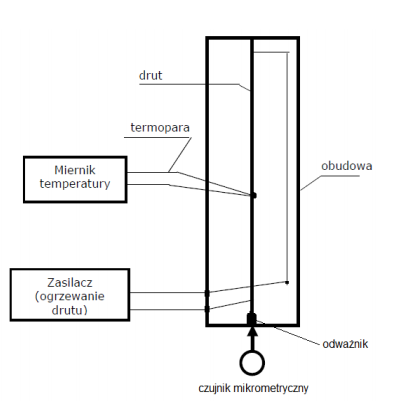
\includegraphics[scale=0.9]{xd.PNG}
    \caption{Schemat układu}
\end{figure}

\section{Opracowanie wyników}
\begin{figure}[h!]
    \centering
    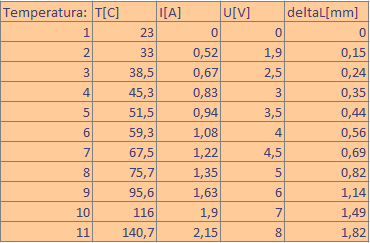
\includegraphics[scale=0.9]{wykresik.PNG}
    \caption{tabela pomiarów}
\end{figure}

\begin{figure}[h!]
    \centering
    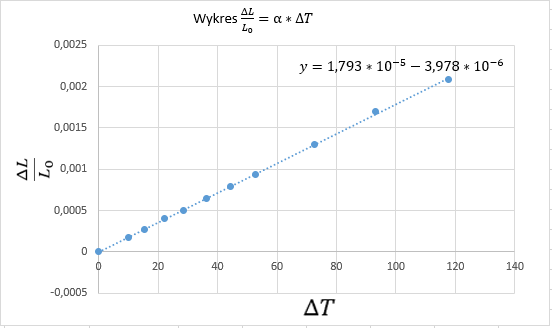
\includegraphics[scale=0.9]{lolo.PNG}
    \caption{Wykres zależności długości od temperatury}
\end{figure}
Niepewności pomiarów oraz ich przykładowe obliczenia:\\

$L_{0}=0,875\pm0,004m$\\

$T_{0}=23\degree C$\\

$\Delta p(L)=0,01mm$\\

$u_{B}(L)=\frac{\Delta p(T)}{\sqrt{3}}\approx5,8\cdot10^{-6}m$\\

$\Delta p(T)=0,05\%+0,5\degree C=\frac{0,05}{100}+0,5=0,5005\degree C$\\

$u_{B}(T)=\frac{\Delta p(C)}{\sqrt{3}}=\frac{0,5005}{\sqrt{3}}\approx0,29\degree C$\\

$\Delta p(I)=1\%+0,01A=\frac{1}{100}+0,01=0,02A$\\

$u_{B}(I)=\frac{\Delta p(I)}{\sqrt{3}}=\frac{0,02}{\sqrt{3}}\approx0,012A$\\

$\Delta p(U)=1\%+0,1V=\frac{1}{100}+0,1=0,11V$\\

$u_{B}(U)=\frac{\Delta p(U)}{\sqrt{3}}=\frac{0,11}{\sqrt{3}}\approx0,064V$\\

$u_{c}\left(\frac{\Delta L}{L_{0}}\right)=\sqrt{\sum^{k}_{j=1}\left(\frac{\partial f}{\partial x_{j}}\right)^{2}\cdot u^{2}(x_{j})}= 
\sqrt{\frac{1}{L_{0}^2}\cdot u_{B}^2(\Delta L)+\frac{\Delta L}{L_{0}^4}\cdot u_{B}^2(L_{0})}\approx 2,3\cdot 10^{-5}m$
\vspace{2.5ex}

Z regresji liniowej wynika, że $\alpha=18\cdot10^{-6}\frac{1}{\degree C}$ natomiast jej błąd wynosi $u(\alpha)=0,15\cdot10^{-6}\frac{1}{\degree C}$
\section{Wnioski}
Po obliczeniu $\alpha$ można wywnioskować, że drut był zrobiony z brązu. Przyrost procentowy drutu rośnie liniowo. 

\end{document}
